% Generated Results figure environments. Requires the manuscript's existing graphicx support.

% Recommended placement: after Block-Period Sensitivity.
\begin{figure}[t]
  \centering
  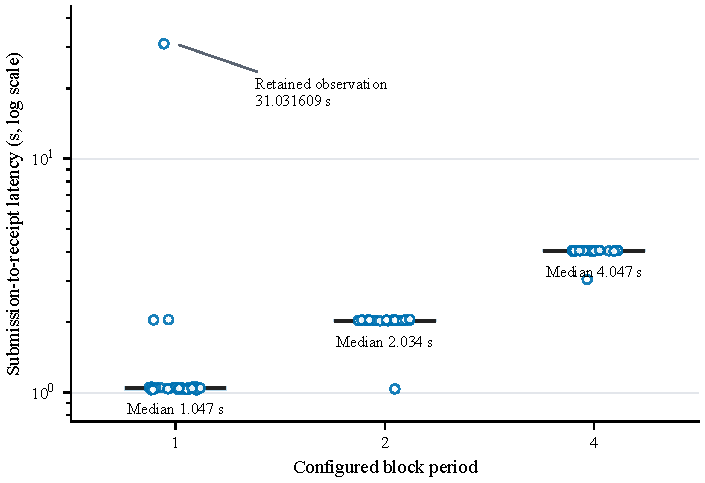
\includegraphics[width=\linewidth]{paper_assets/figures/results/fig_results_block_period_sensitivity.pdf}
  \caption{Submission-to-receipt latency under 1-, 2-, and 4-second configured block periods. Each configuration contains 30 transactions. Individual observations and box summaries are shown on a logarithmic time axis; the retained approximately 31.032-second observation in the 1-second profile remains visible.}
  \label{fig:block-period-sensitivity}
\end{figure}

% Recommended placement: after Main software-fleet outcome table.
\begin{figure}[t]
  \centering
  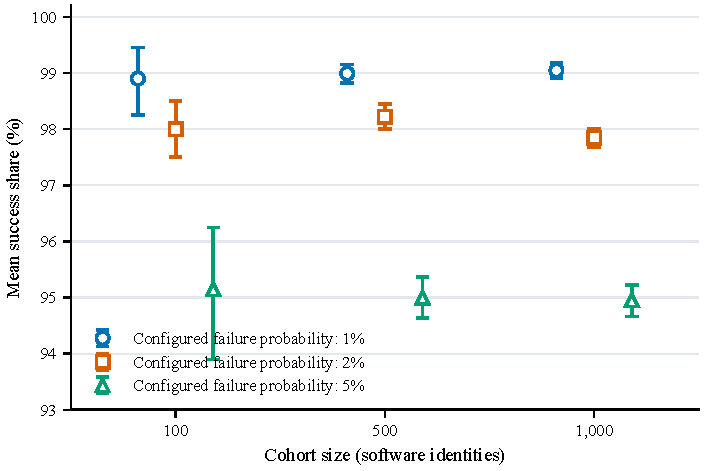
\includegraphics[width=\linewidth]{paper_assets/figures/results/fig_results_success_share_software_cohorts.pdf}
  \caption{Mean success share across authenticated software-cohort configurations. Each point summarizes 20 deterministic seeds for the stated cohort size and configured failure probability; error bars denote bootstrap 95\% confidence intervals.}
  \label{fig:fleet-success-share}
\end{figure}

% Recommended placement: after 500-identity outcome-sensitivity paragraph.
\begin{figure*}[t]
  \centering
  \begin{minipage}[t]{0.32\textwidth}
    \centering
    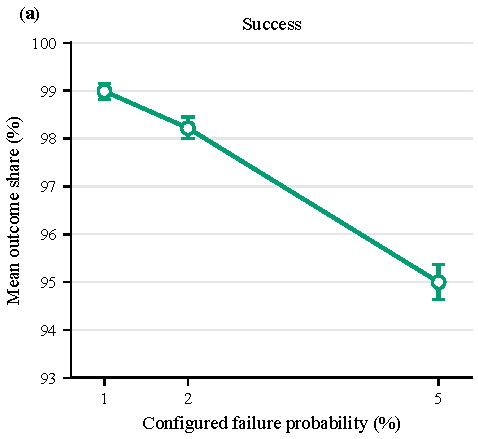
\includegraphics[width=\linewidth]{paper_assets/figures/results/panels/fig_results_failure_probability_sensitivity_a.pdf}
  \end{minipage}%
  \begin{minipage}[t]{0.32\textwidth}
    \centering
    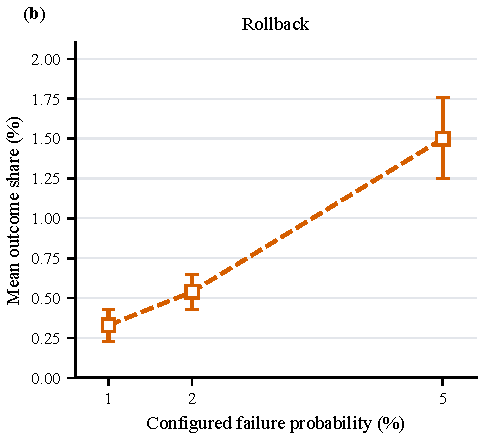
\includegraphics[width=\linewidth]{paper_assets/figures/results/panels/fig_results_failure_probability_sensitivity_b.pdf}
  \end{minipage}%
  \begin{minipage}[t]{0.32\textwidth}
    \centering
    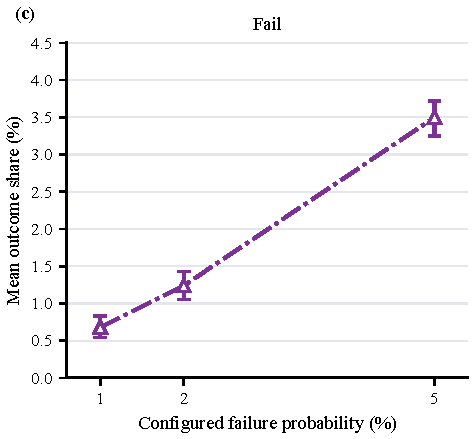
\includegraphics[width=\linewidth]{paper_assets/figures/results/panels/fig_results_failure_probability_sensitivity_c.pdf}
  \end{minipage}\par\smallskip
  \caption{Outcome sensitivity for a 500-identity software cohort. Panels show the mean shares of (a) SUCCESS, (b) ROLLBACK, and (c) FAIL outcomes across 20 deterministic seeds; error bars denote bootstrap 95\% confidence intervals.}
  \label{fig:failure-probability-sensitivity}
\end{figure*}

% Recommended placement: after Retrieval-distribution table.
\begin{figure}[t]
  \centering
  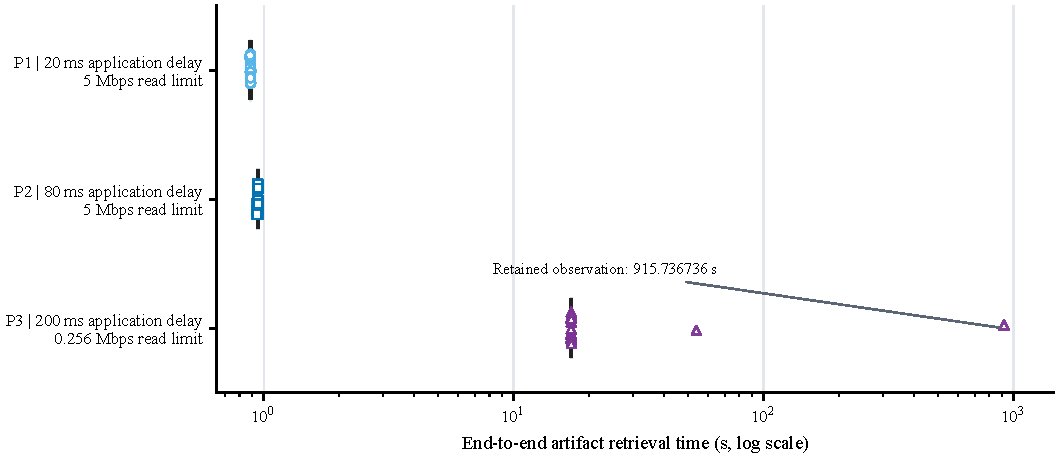
\includegraphics[width=\linewidth]{paper_assets/figures/results/fig_results_application_shaped_ipfs_retrieval.pdf}
  \caption{Application-shaped local IPFS retrieval time for a 537,088-byte artifact. Each profile contains 20 completed transfers shown on a logarithmic time axis. Application-level delays and paced reads were used; all observations were retained, including the 915.737-second observation in P3.}
  \label{fig:ipfs-retrieval}
\end{figure}

% Recommended placement: after Cache summary table.
\begin{figure*}[t]
  \centering
  \begin{minipage}[t]{0.48\textwidth}
    \centering
    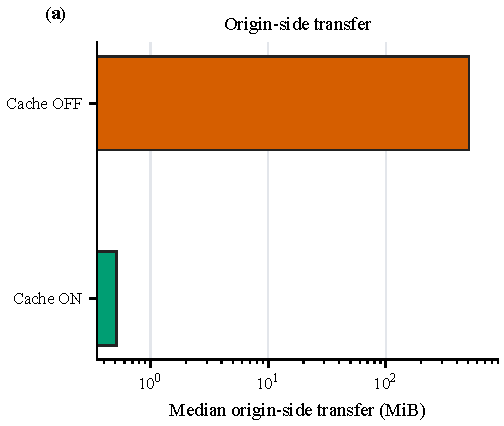
\includegraphics[width=\linewidth]{paper_assets/figures/results/panels/fig_results_local_cache_reuse_a.pdf}
  \end{minipage}%
  \begin{minipage}[t]{0.48\textwidth}
    \centering
    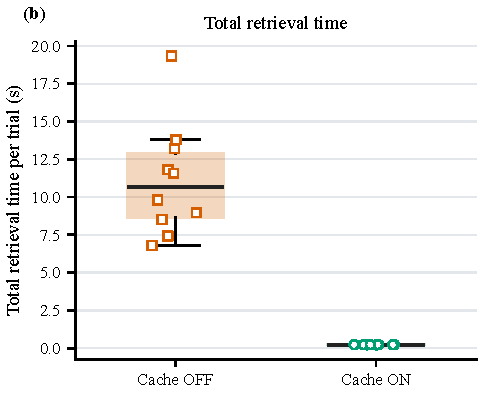
\includegraphics[width=\linewidth]{paper_assets/figures/results/panels/fig_results_local_cache_reuse_b.pdf}
  \end{minipage}\par\smallskip
  \caption{Local cache-reuse ablation across ten independent trials per mode, with 1,000 sequential requests in each trial. Panel (a) reports origin-side transfer, whereas panel (b) shows the distribution of total retrieval time. Each cache-enabled trial began with an empty in-process payload buffer and performed one origin retrieval before serving subsequent requests from the buffer. No integrity failures occurred.}
  \label{fig:cache-reuse}
\end{figure*}

% Recommended placement: after Analytical accountability-sensitivity table.
\begin{figure*}[t]
  \centering
  \begin{minipage}[t]{0.48\textwidth}
    \centering
    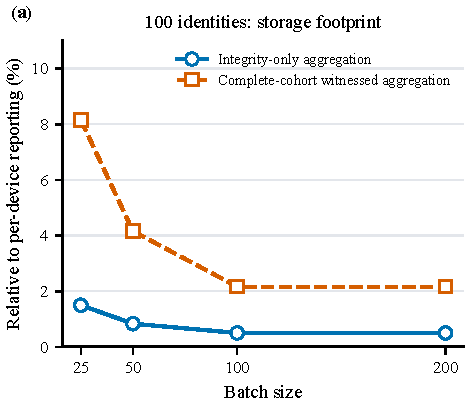
\includegraphics[width=\linewidth]{paper_assets/figures/results/panels/fig_results_storage_bounded_accountability_a.pdf}
  \end{minipage}%
  \begin{minipage}[t]{0.48\textwidth}
    \centering
    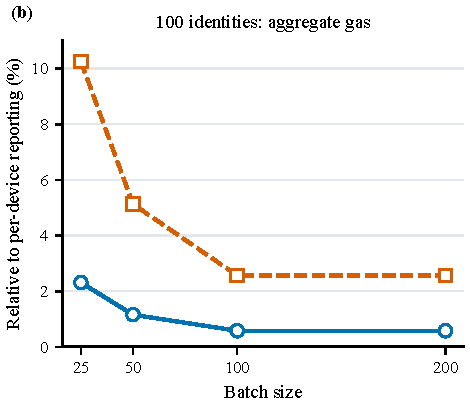
\includegraphics[width=\linewidth]{paper_assets/figures/results/panels/fig_results_storage_bounded_accountability_b.pdf}
  \end{minipage}\par\smallskip
  \begin{minipage}[t]{0.48\textwidth}
    \centering
    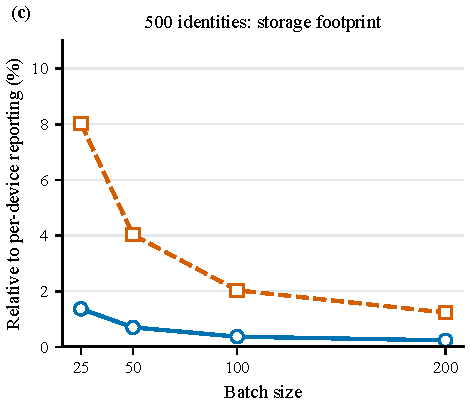
\includegraphics[width=\linewidth]{paper_assets/figures/results/panels/fig_results_storage_bounded_accountability_c.pdf}
  \end{minipage}%
  \begin{minipage}[t]{0.48\textwidth}
    \centering
    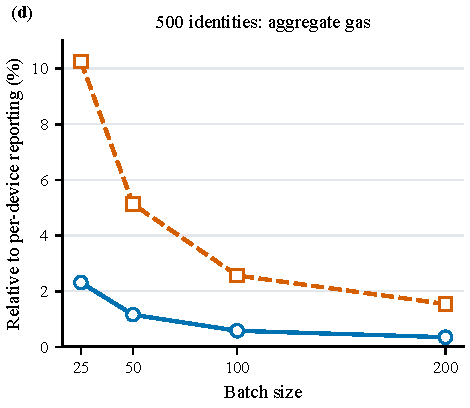
\includegraphics[width=\linewidth]{paper_assets/figures/results/panels/fig_results_storage_bounded_accountability_d.pdf}
  \end{minipage}\par\smallskip
  \begin{minipage}[t]{0.48\textwidth}
    \centering
    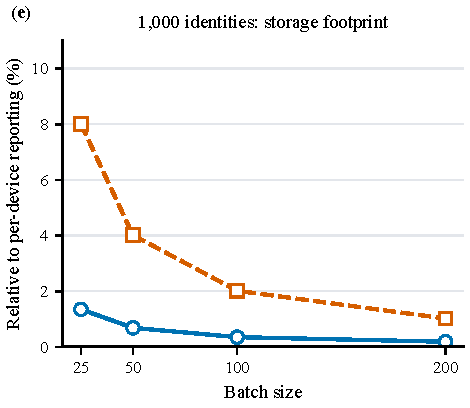
\includegraphics[width=\linewidth]{paper_assets/figures/results/panels/fig_results_storage_bounded_accountability_e.pdf}
  \end{minipage}%
  \begin{minipage}[t]{0.48\textwidth}
    \centering
    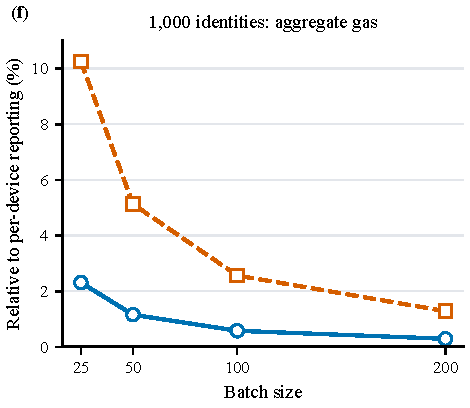
\includegraphics[width=\linewidth]{paper_assets/figures/results/panels/fig_results_storage_bounded_accountability_f.pdf}
  \end{minipage}\par\smallskip
  \caption{Batch-size sensitivity of integrity-only and complete-cohort witnessed aggregation. The left column reports projected on-chain storage footprint and the right column reports projected aggregate gas, each normalized to per-device reporting at 100\%. Rows correspond to cohorts of 100, 500, and 1,000 software identities. Storage values use compiler-reported layouts, whereas gas projections use the executed median logical-path gas for each reporting approach. The per-device 100\% baseline is omitted from the panels to preserve resolution among the aggregation curves.}
  \label{fig:accountability-tradeoff}
\end{figure*}

% Recommended placement: after Crash-fault and restoration table.
\begin{figure*}[t]
  \centering
  \begin{minipage}[t]{0.48\textwidth}
    \centering
    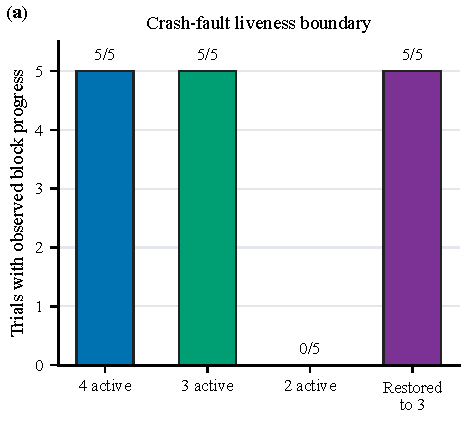
\includegraphics[width=\linewidth]{paper_assets/figures/results/panels/fig_results_validator_crash_faults_a.pdf}
  \end{minipage}%
  \begin{minipage}[t]{0.48\textwidth}
    \centering
    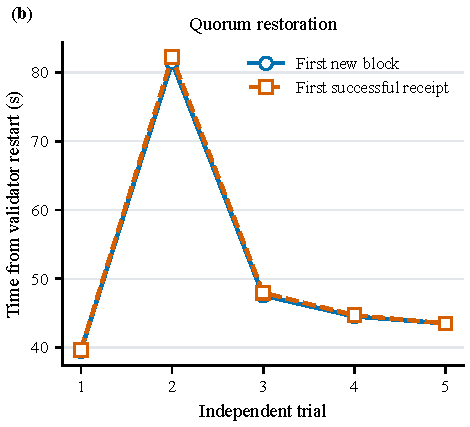
\includegraphics[width=\linewidth]{paper_assets/figures/results/panels/fig_results_validator_crash_faults_b.pdf}
  \end{minipage}\par\smallskip
  \caption{Local validator crash-fault and quorum-restoration results across five independent trials. Panel (a) reports observed block progress with four, three, and two active validators and after restoring a third validator. Panel (b) reports the time from validator restart to the first new block and first successful transaction receipt. The campaign injected process crashes only.}
  \label{fig:validator-faults}
\end{figure*}
